\documentclass[10pt,journal,compsoc]{IEEEtran}
\usepackage{amsmath,bm,mathtools}
\ifCLASSOPTIONcompsoc
  % IEEE Computer Society needs nocompress option
  % requires cite.sty v4.0 or later (November 2003)
  \usepackage[nocompress]{cite}
\else
  % normal IEEE
  \usepackage{cite}
\fi
\ifCLASSINFOpdf
  % \usepackage[pdftex]{graphicx}
  % declare the path(s) where your graphic files are
  % \graphicspath{{../pdf/}{../jpeg/}}
  % and their extensions so you won't have to specify these with
  % every instance of \includegraphics
  % \DeclareGraphicsExtensions{.pdf,.jpeg,.png}
\else
  % or other class option (dvipsone, dvipdf, if not using dvips). graphicx
  % will default to the driver specified in the system graphics.cfg if no
  % driver is specified.
  % \usepackage[dvips]{graphicx}
  % declare the path(s) where your graphic files are
  % \graphicspath{{../eps/}}
  % and their extensions so you won't have to specify these with
  % every instance of \includegraphics
  % \DeclareGraphicsExtensions{.eps}
\fi
% *** MATH PACKAGES ***
%
%\usepackage[cmex10]{amsmath}
% A popular package from the American Mathematical Society that provides
% many useful and powerful commands for dealing with mathematics. If using
% it, be sure to load this package with the cmex10 option to ensure that
% only type 1 fonts will utilized at all point sizes. Without this option,
% it is possible that some math symbols, particularly those within
% footnotes, will be rendered in bitmap form which will result in a
% document that can not be IEEE Xplore compliant!
%
% Also, note that the amsmath package sets \interdisplaylinepenalty to 10000
% thus preventing page breaks from occurring within multiline equations. Use:
%\interdisplaylinepenalty=2500
% after loading amsmath to restore such page breaks as IEEEtran.cls normally
% does. amsmath.sty is already installed on most LaTeX systems. The latest
% version and documentation can be obtained at:
% http://www.ctan.org/tex-archive/macros/latex/required/amslatex/math/

% correct bad hyphenation here
\hyphenation{op-tical net-works semi-conduc-tor}


\begin{document}

\title{A Two-step Kalman/Complementary Filter for Estimation of Vertical Position
Using an IMU-Barometer System}

\author{Jung Keun Lee
\IEEEcompsocitemizethanks{\IEEEcompsocthanksitem Department of Mechanical Engineering, Hankyong
National University
327 Jungang-ro, Anseong, Gyeonggi, 17579, Korea\protect\\
Corresponding author: jklee@hknu.ac.kr}
\thanks{(Received: April 15, 2016; Accepted : May 30, 2016)
This is an Open Access article distributed under the terms of the Creative
Commons Attribution Non-Commercial License(http://creativecommons.org/
licenses/bync/3.0) which permits unrestricted non-commercial use, distribution,
and reproduction in any medium, provided the original work is properly cited.}}

% note the % following the last \IEEEmembership and also \thanks - 
% these prevent an unwanted space from occurring between the last author name
% and the end of the author line. i.e., if you had this:
% 
% \author{....lastname \thanks{...} \thanks{...} }
%                     ^------------^------------^----Do not want these spaces!
%
% a space would be appended to the last name and could cause every name on that
% line to be shifted left slightly. This is one of those "LaTeX things". For
% instance, "\textbf{A} \textbf{B}" will typeset as "A B" not "AB". To get
% "AB" then you have to do: "\textbf{A}\textbf{B}"
% \thanks is no different in this regard, so shield the last } of each \thanks
% that ends a line with a % and do not let a space in before the next \thanks.
% Spaces after \IEEEmembership other than the last one are OK (and needed) as
% you are supposed to have spaces between the names. For what it is worth,
% this is a minor point as most people would not even notice if the said evil
% space somehow managed to creep in.



% The paper headers
\markboth{Journal of Sensor Science and Technology 
Vol. 25, No. 3 (2016) pp. 202-207
http://dx.doi.org/10.5369/JSST.2016.25.3.202
SSN 1225-5475/eISSN 2093-7563}\%
% The only time the second header will appear is for the odd numbered pages
% after the title page when using the twoside option.
% 
% *** Note that you probably will NOT want to include the author's ***
% *** name in the headers of peer review papers.                   ***
% You can use \ifCLASSOPTIONpeerreview for conditional compilation here if
% you desire.



% The publisher's ID mark at the bottom of the page is less important with
% Computer Society journal papers as those publications place the marks
% outside of the main text columns and, therefore, unlike regular IEEE
% journals, the available text space is not reduced by their presence.
% If you want to put a publisher's ID mark on the page you can do it like
% this:
%\IEEEpubid{0000--0000/00\$00.00~\copyright~2014 IEEE}
% or like this to get the Computer Society new two part style.
%\IEEEpubid{\makebox[\columnwidth]{\hfill 0000--0000/00/\$00.00~\copyright~2014 IEEE}%
%\hspace{\columnsep}\makebox[\columnwidth]{Published by the IEEE Computer Society\hfill}}
% Remember, if you use this you must call \IEEEpubidadjcol in the second
% column for its text to clear the IEEEpubid mark (Computer Society jorunal
% papers don't need this extra clearance.)



% use for special paper notices
%\IEEEspecialpapernotice{(Invited Paper)}



\IEEEtitleabstractindextext{%
\begin{abstract}
Estimation of vertical position is critical in applications of sports science
and fall detection and also controls of unmanned aerial vehi- cles and
motor boats. Due to low accuracy of GPS(global positioning system) in the
vertical direction, the integration of IMU(inertial measurement unit) with
the GPS is not suitable for the vertical position estimation. This paper
investigates an IMU-barometer integration for estimation of vertical
position (as well as vertical velocity). In particular, a new two-step
Kalman/complementary filter is proposed for accurate and efficient
estimation using 6-axis IMU and barometer signals. The two-step filter is
composed of (i) a Kalman filter that estimates vertical acceleration via
tilt orientation of the sensor using the IMU signals and (ii) a
complementary filter that estimates ver- tical position using the barometer
signal and the vertical acceleration from the first step. The estimation
performance was evaluated against a reference optical motion capture
system. In the experimental results, the averaged estimation error of the
method was 19.7 cm while that of the raw barometer signal was 43.4
cm.  
\end{abstract}

\begin{IEEEkeywords}
Vertical position, Vertical acceleration, Kalman filter, Complementary filter, IMU(inertial measurement unit), Barometer
\end{IEEEkeywords}}


% make the title area
\maketitle


% To allow for easy dual compilation without having to reenter the
% abstract/keywords data, the \IEEEtitleabstractindextext text will
% not be used in maketitle, but will appear (i.e., to be "transported")
% here as \IEEEdisplaynontitleabstractindextext when the compsoc 
% or transmag modes are not selected <OR> if conference mode is selected 
% - because all conference papers position the abstract like regular
% papers do.
\IEEEdisplaynontitleabstractindextext
% \IEEEdisplaynontitleabstractindextext has no effect when using
% compsoc or transmag under a non-conference mode.



% For peer review papers, you can put extra information on the cover
% page as needed:
% \ifCLASSOPTIONpeerreview
% \begin{center} \bfseries EDICS Category: 3-BBND \end{center}
% \fi
%
% For peerreview papers, this IEEEtran command inserts a page break and
% creates the second title. It will be ignored for other modes.
\IEEEpeerreviewmaketitle



\IEEEraisesectionheading{\section{Introduction}\label{sec:introduction}}


\IEEEPARstart{A}{ccurate} vertical position estimation for moving objects or humans is required
in various fields. For example, in the control of an unmanned aerial vehicle
(UAV) such as a drone, altitude is considered to be a kind of vertical
displacement [1], and vertical displacement such as a skier or snowboard is
required. In the case of severe spots, the vertical displacement estimation
using a portable sensor system can be used for analysis to improve light power
[2]. In order to overcome the space limitations of most motion capture systems
in tracking trajectories of moving objects GPS (global positioning system) IMU
(inertial measurement unit,  Inertial measurement device) has been attempted.
At this time, GPS provides displacement values that do not drift,
and inertial sensors provide high sampling rates, so that high sampling rate
and high accuracy displacement estimation are achieved through fusion of the
two sensors. However, the error of vertical direction displacement of GPS is
about 10 -- 20m, which is much lower than that of horizontal displacement [3]. 

As a countermeasure to this, a barometer can be utilized for vertical
displacement. However, the barometer is very noisy for use alone. Above all,
the barometer estimates the vertical displacement through the sensing of the
atmospheric pressure change. It responds sensitively to atmospheric conditions,
indoor / outdoor conditions, and even the degree of window opening, all of
which cause errors in the calculation of vertical displacement. Thus, similar
to IMU-GPS fusion, barometric-IMU convergence has been studied for
high-sampling rate and high-accuracy vertical displacement estimation [2,4-7].
In particular, IMU-barometer convergence is used in pedestrian navigation [8]
and fall detection [9] in terms of human monitoring.

Two approaches to the IMU and barometric convergence can be considered: tightly
coupled and loosely coupled [5]. The strong coupling method is effective in
modeling the noise of the two signals in a way that the signals of the IMU and
the barometer are fused from the beginning of the filter, but the system matrix
is ​​large and the calculation amount is large. On the other hand,
the weak coupling method uses a two-step filter and is used more frequently
because of convenience of application and efficiency of calculation. In this
case, the two-stage filter computes the vertical displacement using (i) the
first filter to calculate the attitude of the sensor using the IMU signal and
obtain the vertical acceleration through it, and (ii) the vertical acceleration
calculated from the barometer signal and the previous filter The second filter. 


Zihajehzadeh et al. [2] proposed a Kalman filter (KF) [10], which uses a 6-axis
IMU developed by this author (ie, a 3-axis accelerometer and a 3-axis
gyroscope) , And the Kalman filter, which sets the vertical displacement and
the vertical velocity as state variables, was used as the second filter.
Tanigawa et al. [7] applied the same Kalman filter as the first filter to the
Xsens three-dimensional posture calculation based on the 9-axis IMU (ie 6-axis
IMU + 3-axis geomagnetic sensor) All. Meanwhile, Sabatini and Genovese [5]
proposed an extended Kalman filter (Extended KF, EFK) that obtains quaternions
using 6-axis IMU As a first filter, use a complementary filter (CF) The second
filter was used. In addition, Son and Oh proposed [4] The EKF has claimed that
the IMU can be calibrated during the measurement by adding the accelerometer
bias and scale factor in addition to the vertical displacement and vertical
velocity as state variables, thereby improving the accuracy of posture and
vertical displacement estimation.

Among the above methods, all methods except [5] use a Kalman filter as the second filter,
for smoothing and smoothing effects.  However, the Kalman filter has a
disadvantage that the calculation amount is larger than that of the
complementary filter.

In this paper, the accurate vertical acceleration is estimated by using the
tilt estimation Kalman filter [10] adopted in [2] as the first filter, and a
new combination IMU - Barometer based

A two-stage Kalman / complementary filter is proposed. In addition, (1) the
effect of the accuracy of vertical acceleration estimation on the accuracy of
vertical displacement estimation in (1), and (2) the comparison between short
and long endpoints and estimation accuracy based on the complementary filter
and Kalman filter selection in the second stage. In this paper, we propose an
optimal vertical displacement estimation filter that combines the accuracy of
estimation and calculation efficiency.

\section{Estimation algorithm and verification experiment}

\subsection{Kalman filter for vertical acceleration estimation via posture estimation}

The Kalman filter for vertical acceleration estimation, which is the first
step, estimates the tilt as a vertical axis slope using an accelerometer and
gyroscope signal, which is a 6-axis IMU [10], and compensates for the
gravitational acceleration component in the accelerometer signal (See Fig. 1).

The signals of the gyroscope (G) and the accelerometer (A) were modeled as
follows:

\[\bm{s}_G = \prescript{S}{}{\bm{\omega}}+\bm{n}_G\tag{1.a}\]

\[\bm{s}_A = \prescript{S}{}{\bm{g}}+\prescript{S}{}{\bm{a}}+\bm{n}_G\tag{1.b}\]


\noindent where $\bm{\omega}$ is the angular velocity, $\bm{a}$ is the sensor acceleration and $\bm{n}$ is the
measurement noise. The superscript $S$ also means that the vector is represented
in the sensor coordinate system. In equation (1.b), the sensor acceleration is
modeled as a first-order Markov chain process:

\[\prescript{S}{}{\bm{a}_t} = c_a\prescript{S}{}{\bm{a}_{t-1}}+\bm{\varepsilon}_{a,t}\tag{2}\]

\noindent where $c_a$ and $\bm{\varepsilon}_{a,t}$ are constant parameters and time-varying error terms of
the acceleration model, respectively.

The first filter estimates the tilt attitude expressed by
$\prescript{S}{}{\bm{Z}}$ as a state vector, and obtains the vertical
acceleration through the estimation. Where $\prescript{S}{}{\bm{Z}}$ is a
representation of the Z-axis unit vector of the inertial coordinate system I in
the sensor coordinate system and is part of a direction cosine matrix which is
a three-dimensional attitude matrix. First, the process model that updates the
state variable $x_1 (= \prescript{S}{}{\bm{Z}})$ over time is expressed as
follows from the strapdown integration associated with the angular velocity
measurement of the gyroscope:

\[\bm{x}_{1,t}=\prescript{S}{}{\bm{Z}_t}=
(\bm{I}-\Delta t\bm{\tilde{s}}_{G,t-1})\prescript{S}{}{\bm{Z}_{t-1}}+\Delta t(-\prescript{\tilde{S}}{}{\bm{Z}_{t-1}})\bm{n}_G\tag{3}\]

Here, $\Delta t$ is the sampling interval and the tilde ($\tilde{~}$) denotes the outer matrix of
the vector, e.g., $\tilde{a} = [a \times]$.

The measurement model is a mixture of accelerometer signal and sensor acceleration model as follows:

\[\bm{s}_{A,t}-c_a\prescript{S}{}{\bm{a}^+_{t-1}}=g\prescript{S}{}{\bm{Z_t}}\prescript{S}{}{\bm{a}^-_{\varepsilon,t}}+\bm{n}_A\tag{4}\]


The following relation is applied in the above equation: 
$\prescript{S}{}{\bm{g}} = g\prescript{S}{}{\bm{Z}}$, 
$\prescript{S}{}{\bm{a}^-_{\varepsilon,t}} = \prescript{S}{}{\bm{a}^-_t} - \prescript{S}{}{\bm{a}_t}$, 
The superscripts $-$ and + mean the a priori and the posteriori, respectively.

From the equations (3) and (4) we obtain the following KF equation:

(5.a)

(5.b)

where the transition matrix Φ t - 1 is I - Δ ts G, t - 1; The process noise w t
- 1 is Δ t (- Z t - 1) n G; The measurement vector z t is s A, t - c a a t - 1;
The observation matrix H t is gI; And the measurement noise v t is - a ε, t + n
A. The covariance matrix, Q t - 1 (= E [w t - 1 - w t - 1]) and M t (= E [v t v
t]) for the progressive noise and the measured noise are as follows.

(6.a)

(6.b)

where E is the expectation operator, the covariance matrix Σ G for gyro
measurement noise is σ GI 3, the covariance matrix Σ A for accelerometer
measurement noise is set to σ AI 3, and σ G and σ A are noise standard
deviations. The covariance matrix Σ acc of the acceleration model error defined
by E ((ε, t) (a ε, t)) is set to 3 caat - 1 I.

Once Z is obtained, the external acceleration a from the viewpoint of the
sensor coordinate system is obtained as s A - g Z, and finally the Z-direction
acceleration a z from the viewpoint of the inertial coordinate system is
obtained by the following equation.

(7)


\begin{figure}[!t]
\centering
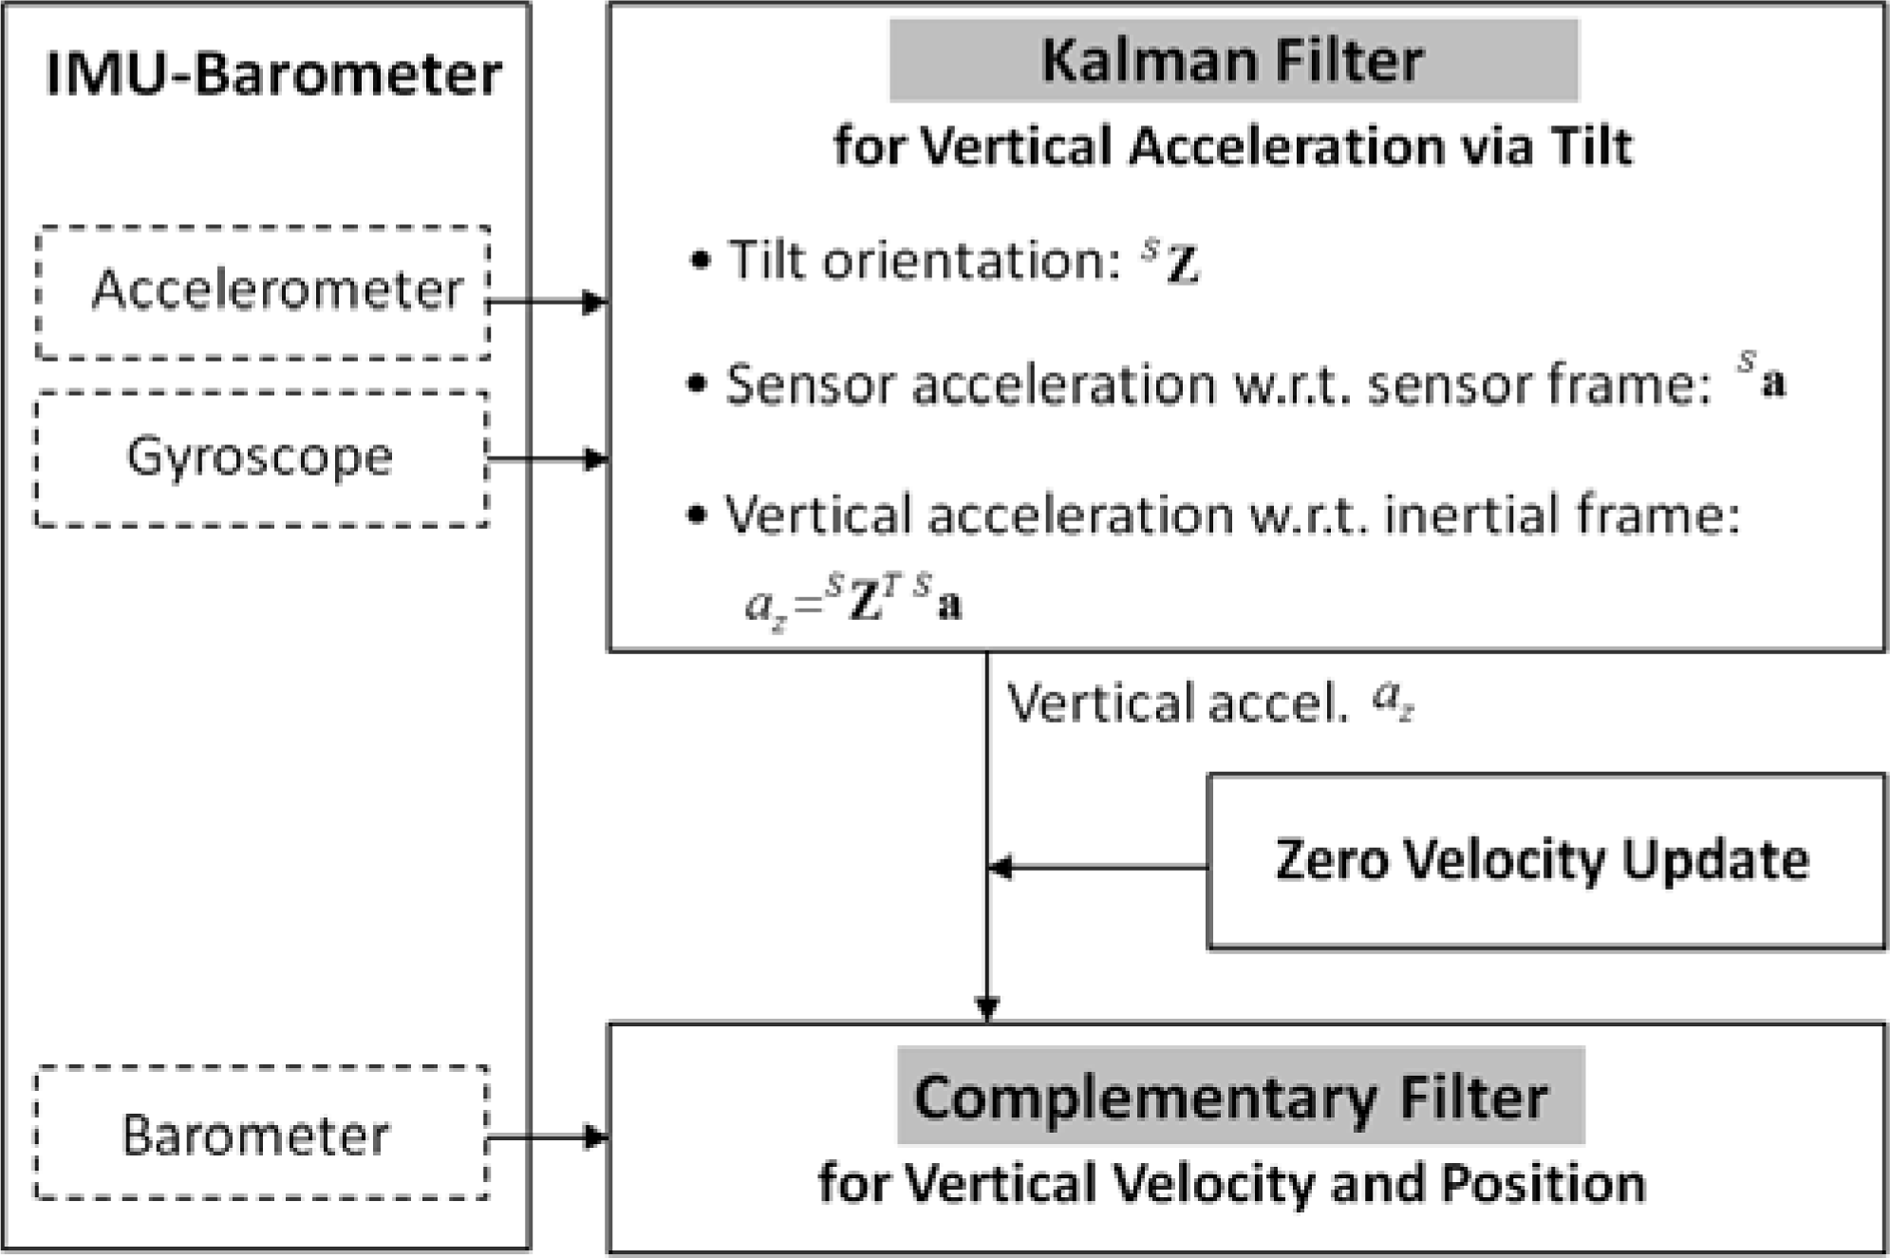
\includegraphics[width=2.5in]{fig1}
    \caption{Flowchart of the proposed two-step Kalman/complementary filter.}
\label{fig1}
\end{figure}

\subsection{Complementary filter for vertical displacement estimation}


In the second step, a complementary filter, the vertical displacement h z (= h
z) and the vertical velocity v z (= v z) are estimated using the vertical
acceleration transmitted through the first Kalman filter and the barometric
signal.

The barometer pressure P can be converted to the vertical displacement h z by
the following equation [12].

(8)

\section{Conclusion}
The conclusion goes here.

\appendices
\section{Proof of the First Zonklar Equation}
Appendix one text goes here.

% you can choose not to have a title for an appendix
% if you want by leaving the argument blank
\section{}
Appendix two text goes here.


% use section* for acknowledgment
\ifCLASSOPTIONcompsoc
  % The Computer Society usually uses the plural form
  \section*{Acknowledgments}
\else
  % regular IEEE prefers the singular form
  \section*{Acknowledgment}
\fi


The authors would like to thank...


% Can use something like this to put references on a page
% by themselves when using endfloat and the captionsoff option.
\ifCLASSOPTIONcaptionsoff
  \newpage
\fi



\begin{thebibliography}{1}

\bibitem{IEEEhowto:kopka}
H.~Kopka and P.~W. Daly, \emph{A Guide to \LaTeX}, 3rd~ed.\hskip 1em plus
  0.5em minus 0.4em\relax Harlow, England: Addison-Wesley, 1999.

\end{thebibliography}


\end{document}
